\chapter{Presupuesto y control}

\section{Presupuesto y retorno de la inversión}

\begin{figure}[htb]
\centering
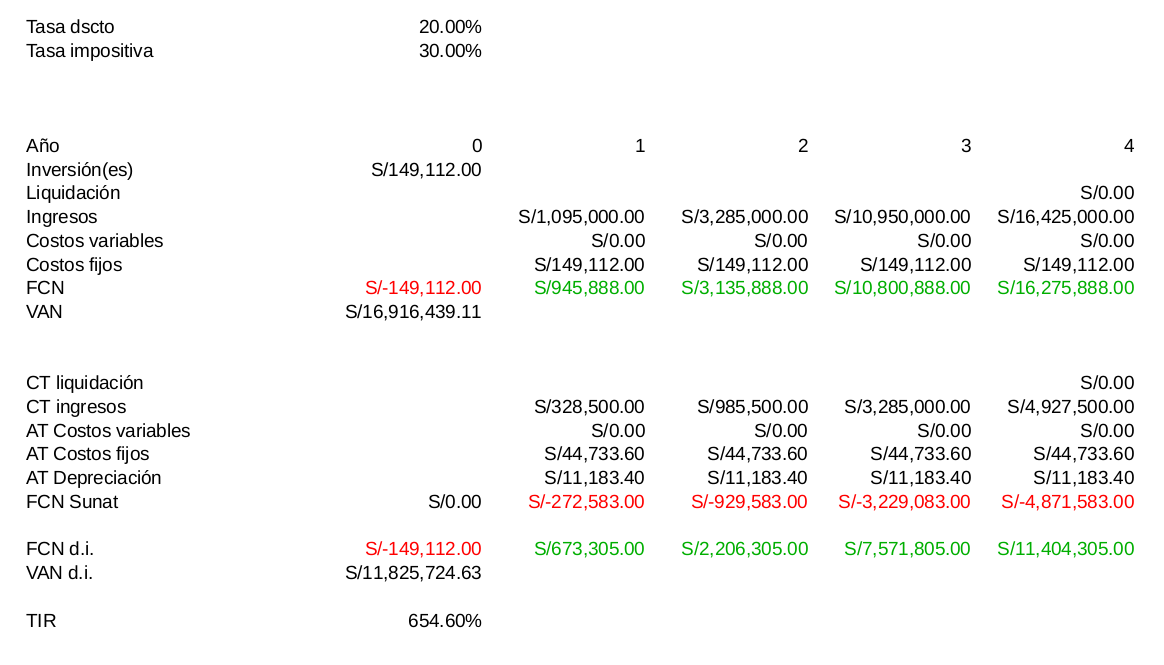
\includegraphics[width=0.8\textwidth]{./img/van_tir}
\caption{Cálculo del VAN y el TIR} \label{fig:van_tir}
\end{figure}

Para calcular el VAN (Valor Actual Neto) y el TIR (Tasa Interna de Retorno), asumimos la siguiente información. La duración del proyecto será de 4 años. En primer lugar, no tenemos costos variables, sólamente costos fijos. La suma de nuestros costos fijos (ver sección \ref{sec:costos}) es de S/. 149 112 anuales. Tomamos como inversión inicial esta misma cifra, pues no hace falta comprar equipo especial al inicio del proyecto (se asume que los trabajadores tienen sus propias herramientas de desarrollo).

Para calcular los ingresos, es muy importante el dato de que hay más de 30 mil taxis en Arequipa. Para efectos prácticos nosotros redondeamos esta cifra a 30 mil exactos. Nuestra proyección de crecimiento nos dice que durante el primer año, un 2\% de taxistas utilizarán nuestra aplicación, para el segundo año serán un 6\%, y para el tercer y cuarto año serán un 20\% y 30\% respectivamente. Luego, el número promedio de carreras diarias de un taxista es de 10. Si cobramos una comisión equivalente a S/. 0.50 por cada carrera, entonces nuestra ganancia promedio al día por taxista que usa nuestra aplicació es de S/. 5.00. Tomaremos como ejemplo el primer año, donde deberíamos tener el 2\% de taxistas trabajando con nosotros, eso es un total de 600 taxistas. Luego, las ganancias por taxista son de S/. 5 diarios que multiplicado por los 600 taxistas y los 365 días del año nos da un bonito S/. 1 095 000.00 que son los ingresos del primer año. Los ingresos de los años siguientes se calculan de forma análoga.

Asumimos una tasa impositiva de 30\% y una tasa de descuento de 20\% para calcular el VAN. El resto sólo son fórmulas.

\section{Cronograma de implementación}

\begin{figure}[htb]
\centering
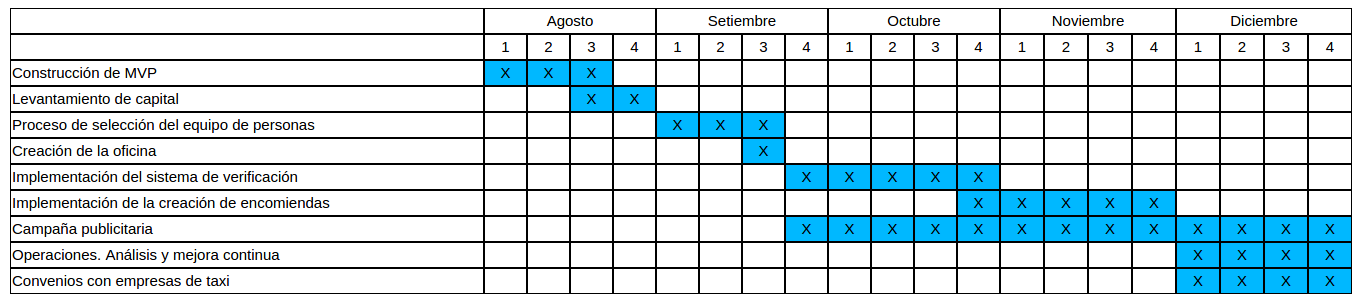
\includegraphics[width=1\textwidth]{./img/cronograma}
\caption{Cronograma de implementación} \label{fig:cronograma}
\end{figure}

El cronograma se encuentra bosquejado en la figura \ref{fig:cronograma}. El plan a grandes rasgos es crear rápidamente un MVP para poder levantar inversiones y lanzar el proyecto. Buscar al resto de las personas del equipo, que por ahora sólo somos dos fundadores y centrarnos durante dos meses en las dos partes más críticas del sistema: la verificación de la identidad de los taxistas y el servicio de courier propiamente dicho. Luego de esto se inicia una campaña de marketing agresiva y se trata de hacer convenios con las empresas de taxi más reconocidas. A la par, se mantiene una cultura de constante análisis y mejora dentro de la empresa, de forma que nos podamos mantener innovando.


\section{Mecanismos de control}